%!TEX root = ../thesis.tex

\section{本章の概要}

本章では,2章で述べたようにロボットの行動を考慮した歩行者の軌道予測を行う手法を提案する.歩行者の軌道予測に関する問題設定を3.2章,学習に用いたネットワーク構造を3.3章,ロボットの行動を考慮した軌道予測する方法を3.4章,ネットワークの学習方法を3.5章,及び学習環境を3.6章,ネットワークの予備実験の内容を3.7章でそれぞれ述べる.

% 以下では,予測を行うネットワーク構造とその学習方法に関して説明する.

% 〜について目指す.〜について提案する.

\section{問題設定}
本論文における歩行者のグラフ表現を説明する.時刻$t$におけるシーン内の歩行者の位置を表す空間グラフを$G_t = (V_t, E_t)$と定義する.ここで,$V_t = \{ v^i_t \mid i = 1, \dots N \}$はグラフ$G_t$のノードの集合であり,各ノード$v^i_t$は$i$番目の歩行者の位置$(x^i_t, y^i_t)$を属性として持つ.$E_t = \{ e^{ij}_t \mid i, j = 1, \dots N \}$はグラフ$G_t$のエッジの集合であり,$e^{ij}_t$はノード$v^i_t$と$v^j_t$が接続されている場合1,そうでない場合0の値をとる.

人間の軌道予測は,歩行者の将来の2次元空間の$x,y$座標を,事前観測の情報を与えて予測ステップ分出力することである.
ここで,歩行者$i$の各時刻の位置を
\begin{equation}
  V_t = \{ v^i_t = (x^i_t, y^i_t) \in \mathbb{R}^2 \mid i = 1, \dots N \}
\end{equation}
と表す.また,$t_{obs}$を観測時間としたとき,観測された全歩行者の位置データを
\begin{equation}
  V_{obs} = \{ V_t \mid t = 1, \dots t_{obs} \}  
\end{equation}
と表す.ここで,時刻$t$の2次元空間における歩行者$i$の位置の確率分布を
\begin{equation}
  \hat{V}_t = \{ \hat{p}^i_t = (\hat{x}^i_t, \hat{y}^i_t) \mid i = 1, \dots N \} \label{hat-pos}
\end{equation}
と表す.$t_{pred}$を予測時間としたとき,予測する全歩行者の位置データを
\begin{equation}
  V_{pred} = \{ \hat{V}_t \mid t = t_{obs + 1}, \dots t_{pred} \}
\end{equation}
と表すことができる.$p^i_t$が$\mathcal{N}(\mu^i_t, \sigma^i_t, \rho^i_t)$となる2変量ガウス分布に従うと仮定する.すなわち,$\hat{p}^i_t$は平均$\hat{\mu}^i_t$,分散$\hat{\sigma}^i_t$,相関係数$\hat{\rho}^i_t$を持つガウス分布
\begin{equation}
  \hat{p}^i_t \sim \mathcal{N}(\hat{\mu}^i_t, \hat{\sigma}^i_t, \hat{\rho}^i_t)
\end{equation}
に従う.ここで,平均を$\hat{\mu}^i_t = (\hat{\mu}^i_{x, t}, \hat{\mu}^i_{y, t})$,分散を$\hat{\sigma}^i_t = (\hat{\sigma}^i_{x, t}, \hat{\sigma}^i_{y, t})$とする.

\section{ネットワーク構造}
本手法で用いられるネットワークは,エンコーダ・デコーダ構造で構成されている.ネットワークは,主にエンコーダモジュール,グラフアテンションネットワークモジュール,デコーダモジュールから構成される.エンコーダモジュールでは,入力データから特徴量を抽出し,グラフアテンションネットワークを用いて,ノード間の関係性を学習する.これらの潜在表現を基に,デコーダモジュールで目的のシーケンス長の予測を行う.
\figref{Fig:network}は,このネットワークの概要を表している.

\begin{figure}[hbtp]
  \centering
 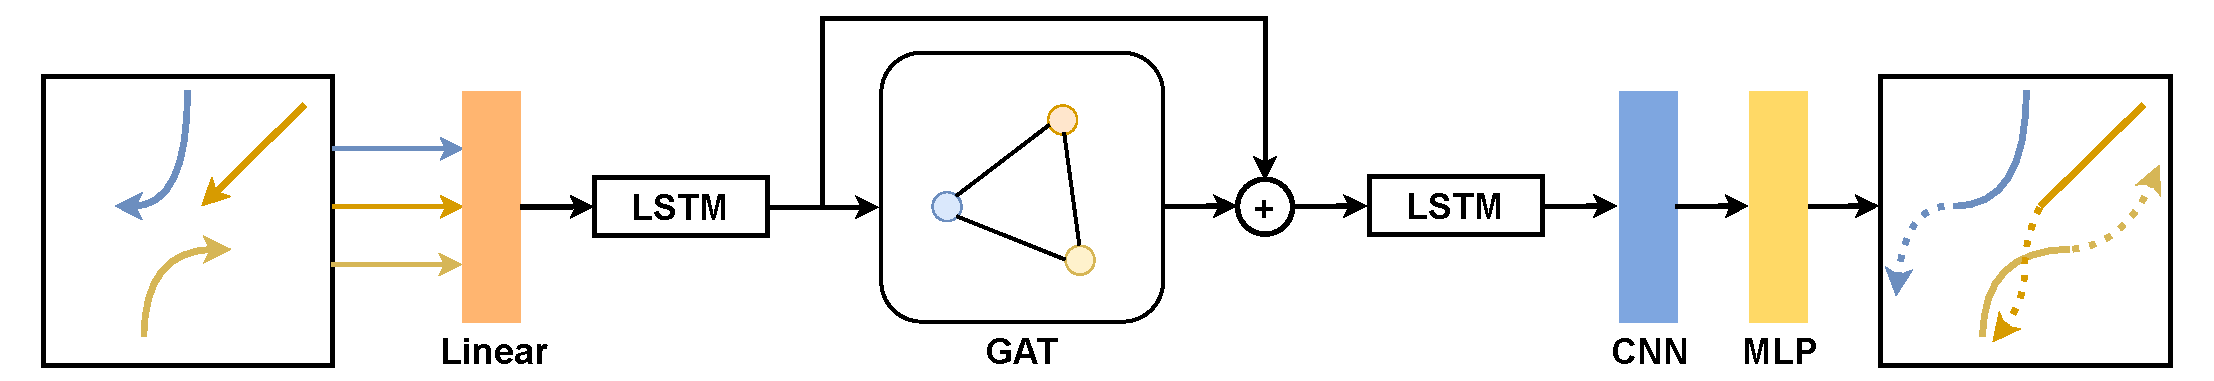
\includegraphics[keepaspectratio, scale=0.36]
      {images/network-comp.pdf}
 \caption{Network Structure}
 \label{Fig:network}
\end{figure}   

\subsection{エンコーダモジュール}
エンコーダでは,まず,入力の各時刻における歩行者の過去の位置は,線形変換層$\phi_{emb}$を用いて高次元空間に埋め込まれる.この埋め込み表現は,LSTM層に入力され,歩行者の過去の位置情報を時間的に処理し,隠れ状態を出力する.隠れ状態は,歩行者の過去の動きを要約したものであり,次のグラフアテンションネットワークに渡される.エンコーダでの処理を式\eqref{emb},\eqref{lstm-en}に示す.なお,$v^i_t \text{と} v^t_i$は等価である.
\begin{align}
  e^t_i &= \phi_{emb}(v^t_i ; W_{emb}) \label{emb} \\
  h_i &= \text{LSTM}_{en}(e^t_i, h^{t-1}_i ; W_{en}) \label{lstm-en}
\end{align}

\subsection{グラフアテンションネットワーク}
ネットワークの中核を担うグラフアテンションネットワーク(GAT)\cite{velickovic2017graph-gat}は,複数層で構成される.各GAT層は,マルチヘッドアテンション機構を用いて,各ノードの特徴をその近傍ノードの特徴と集約する.アテンション機構は,ノード間の関係の強さに基づいて重み付けを行うため,より関連性の高いノードからの情報が強調される.本ネットワークでは,複数のGAT層を積み重ねることで,グラフ構造における高次の依存関係を捉えることができる.各タイムステップにおいて,対応する隣接行列を用いてグラフ畳み込みが実行され,動的なグラフ構造の変化にも対応できる.

歩行者$i$の隠れ状態$h_i$が与えられたとき,全ての歩行者に対して,複数のGAT層を適用する.各層は以下のように適用される.式\eqref{gat-eij}は,ノード$i$に対するノード$j$の特徴の重要度を表している.$W$は重み行列であり,$a$は共有アテンション機構である.また,$\sigma$は活性化関数であり,本手法ではネットワーク全体でPReLU\cite{he2015delving-prelu}を用いた.
\begin{align}
  e_{ij} = a(Wh_i, Wh_j) \label{gat-eij} \\
  \alpha_{ij} = \text{softmax}_{j}(e_{ij}) \\
  h'_i = \sigma\Bigg(\sum_{j \in \mathcal{N}_i} \alpha_{ij}Wh_j \Bigg)
\end{align}

\subsection{デコーダモジュール}\label{sec:decoder}
GAT層からの出力は,デコーダモジュールによって将来の歩行者の予測位置に変換される.まず,2つ目のLSTM層がGATによって生成された時空間特徴表現をさらに時間的に処理する.次に,1次元畳み込み層を用いて,入力シーケンス長から予測シーケンス長への変換が行われる.この層は,予測時間に合わせて特徴表現を調整する役割を果たす.最後に多層パーセプトロン(MLP)が予測値を生成する.式\eqref{output}のように,ネットワークの最終的な出力は5次元である.なお,$\hat{P}^t_i\text{と}\hat{P}^i_t$は等価である.
\begin{align}
  h''_i = \text{LSTM}_{dec}(h'_i, h_{deci}; W_{dec})\\
  c^t_i = \text{CNN}(h''_i; W_{cnn}) \\
  \hat{P}^t_i = \text{MLP}_{d}(c^t_i; W_{d}) \\
  \hat{P}^i_t = [\hat{\mu}^i_{x,t}, \hat{\mu}^i_{y, t}, \hat{\sigma}^i_{x, t}, \hat{\sigma}^i_{y, t}, \hat{\rho}^i_t] \label{output}
\end{align}

さらに,本ネットワークでは\figref{Fig:network}のように,GAT層とLSTM層の出力にスキップ接続\cite{he2016deep-resnet}を導入することで,勾配消失問題\cite{hochreiter2001gradient-grad,weinleindiplomarbeit-grad, schmidhuber2015deep-grad}を軽減し,学習を安定化させる.このアーキテクチャにより,時系列データの動的な変化とグラフ構造におけるノード間の複雑な関係を効果的に捉え,高精度な予測を実現する.

\section{ロボットの行動を考慮した軌道予測}
% 先行研究\cite{si2023-tanno}と同様に,予測時間においてロボットが詮索する予定の経路を予測に用いることが本研究のテーマだが,

歩行者が頻繁に行き交うような環境において,低速域で走行する移動ロボットの行動が歩行者の行動と近似できるという仮定を前提とする.つまり,ロボットと歩行者を区別せずに予測を行う.
ロボットの行動を考慮した軌道予測を行うために,ロボットの経路情報を追加の入力としてネットワークに与える.具体的には,ロボットの位置情報を歩行者の位置情報と同様にグラフのノードとして扱い,エンコーダモジュールで処理する.これにより,ロボットと歩行者の相互作用を考慮した予測が可能となる.

ロボットの位置を表すノード$r_t$を追加し,グラフ$G_t$を拡張する.拡張されたグラフ$\tilde{G}_t = (\tilde{V}_t, \tilde{E}_t)$は,$\tilde{V}_t = V_t \cup \{ r_t \}$と定義される.エッジ集合$\tilde{E}_t$も同様に拡張され,ロボットと歩行者間のエッジが追加される.なお,拡張されたグラフ$\tilde{G}_t$は,ネットワーク構造を変更せずに入力することができる.

エンコーダモジュールでは,ロボットの位置$r_t$も他のノードと同様に埋め込み表現$e^t_r$に変換され,LSTM層に入力される.グラフアテンションネットワークでは,ロボットと歩行者間の相互作用を考慮したアテンション重みが計算される.デコーダモジュールでは,ロボットの位置情報を含む潜在表現を基に,将来の歩行者の位置を予測する.
このようにして,ロボットの行動を考慮した軌道予測を実現する.\ref{chap:experiments_oculus}章では,実験で提案手法の有効性を評価する.

\section{学習方法}\label{sec:learning-method}
提案するネットワークの学習方法の詳細について述べる.
ネットワークは,負の対数尤度を最小化するように学習される.損失関数を式に示す.
\begin{equation}
  L^i = -\sum_{t=t_{obs+1}}^{t_{pred}} \log \left( P(\hat{p}^i_t \mid \hat{\mu}^i_t, \hat{\sigma}^i_t, \hat{\rho}^i_t) \right)
\end{equation}

このネットワークは,2つの歩行者の軌跡データを含むデータセットで学習される.ETHデータセット\cite{pellegrini2009you-eth}とUCYデータセット\cite{lerner2007crowds-ucy}である.この2つのデータセットには,図のような5つのシーンがあり,計1536人の歩行者のデータが含まれている.5つのシーンは,ETH,HOTEL,UNIV,ZARA1,ZARA2から構成されている.データセットの軌跡は0.4秒ごとにサンプリングされたものである.

\begin{figure}[hbtp]
  \centering
 \includegraphics[keepaspectratio, scale=0.5]
      {images/RaspberryPiMouse.png}
 \caption{Neural Network}
 \label{Fig:hoge4}
\end{figure}

\newpage

\section{学習環境}
本研究で行う学習は全て以下の\tabref{tab:environment}に示す環境で実施する.

\begin{table}[hbtp]
  \centering
  \caption{Experimental Setup}
  \label{tab:environment}
  \begin{tabular}{ll}
    \hline
    OS & Ubuntu 20.04.6 LTS \\
    CPU & Intel Core i7-10700F \\
    GPU & NVIDIA GeForce RTX 3060 \\
    Memory & 32GB \\
    Language & Python 3.8.10 \\
    Flamework & PyTorch 2.4.1 \\
    \hline
  \end{tabular}
\end{table}

\section{ネットワークの予備実験}
ロボットの行動を考慮した軌道予測が行えるか実験で確認する前に,提案したネットワークの性能を確認するため,予備実験を行った.

\subsection{実験概要}
この実験では,Mohamedら\cite{s-stgcnn}の実験方法に倣って,訓練済みモデルを後述する2種類の指標により評価する.その結果を複数のベースラインモデルと比較する.

\subsection{学習条件}
ネットワークの学習は,先行研究\cite{s-lstm,s-stgcnn}と同様の方針に従い,リーブワンアウト(Leave One Out)方式を採用する.これにより,データセットを最大限に活用することができる.
具体的には,5つのシーンの内,1つのシーンをテストデータとして取り除き,残りのデータを用いてモデルを訓練・検証する.テスト時には,8ステップにあたる3.2秒間観測し,次の12ステップにあたる4.8秒間を予測する.学習パラメータは,バッチサイズを128,Adam\cite{kingma2014adam}を用いて250エポック分の学習を行った.学習率は0.001である.

\subsection{評価指標}
モデルの評価には,以下の2つの指標を用いた.

\begin{itemize}
  \item \textbf{ADE(Average Displacement Error)}\cite{pellegrini2009you-eth}:
    \begin{align}
      \text{ADE} = \frac{1}{TN} \sum_{t=1}^{T} \sum_{i=1}^{N} \| p^i_t - \hat{p}^i_t \|_2
    \end{align}
    ここで,$p^i_t$ は時刻 $t$ における歩行者 $i$ の実際の位置,$\hat{p}^i_t$ は予測された位置,$N$ は歩行者の総数,$T$ は予測の総時間ステップである.なお,本研究では$T = 12$である.ADEは,\figref{fig:ade}に示すように,予測された位置と実際の位置との平均的な距離誤差を示す指標である.
    \\
    \item \textbf{FDE(Final Displacement Error)}\cite{s-lstm}:
    \begin{align}
      \text{FDE} = \frac{1}{N} \sum_{i=1}^{N} \| p^i_t - \hat{p}^i_t \|_2 , \ t = t_{pred}
    \end{align}
    ここで,$p^i_t$ は最終時刻 $t_{pred}$ における歩行者 $i$ の実際の位置,$\hat{p}^i_t$ は予測された位置である.FDEは,\figref{fig:fde}に示すように,予測の最終時刻における位置と実際の位置との間の距離誤差を示す指標である.
\end{itemize}

\begin{figure}[hbtp]
  \centering
  \begin{minipage}{0.49\textwidth}
    \centering
    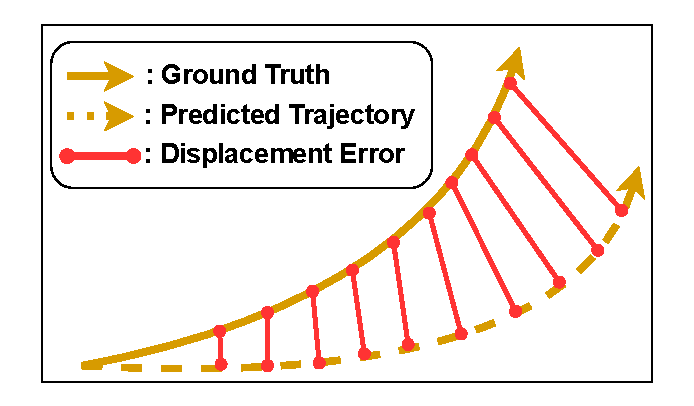
\includegraphics[width=\textwidth]{images/ade.pdf}
    \caption{ADE}
    \label{fig:ade}
  \end{minipage}
  \hfill
  \begin{minipage}{0.49\textwidth}
    \centering
    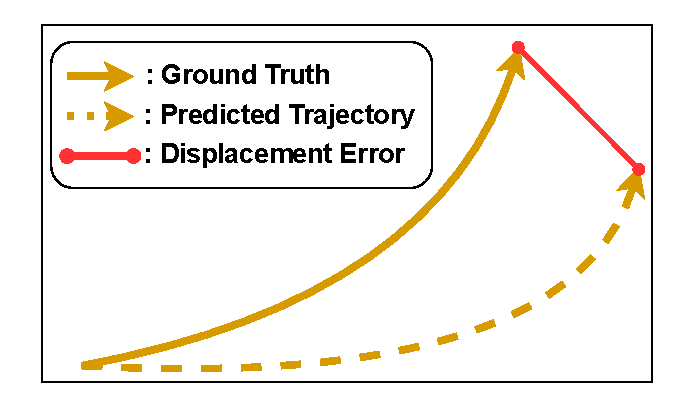
\includegraphics[width=\textwidth]{images/fde.pdf}
    \caption{FDE}
    \label{fig:fde}
  \end{minipage}
\end{figure}

\newpage

\subsection{結果と考察}
\begin{table}[hbtp]
  \centering
  \caption{Comparison of ADE/FDE for each model\protect\footnotemark[6]}
  \label{tab:val-results}
  \footnotesize
  \begin{tabular}{c||c|c|c|c|c|c}
  Model & ETH & HOTEL & UNIV & ZARA1 & ZARA2 & Average \\
  \hline \hline
  Linear \cite{s-lstm} & 1.33/2.94 & 0.39/0.72 & 0.82/1.59 & 0.62/1.21 & 0.77/1.42 & 0.79/1.59 \\
  \hline
  SR-LSTM-2 \cite{sr-lstm} & 0.63/1.25 & 0.37/0.74 & 0.51/1.10 & 0.41/0.90 & 0.32/0.70 & 0.45/0.94 \\
  \hline
  S-LSTM \cite{s-lstm} & 1.09/2.35 & 0.79/1.76 & 0.67/1.40 & 0.47/1.00 & 0.56/1.17 & 0.72/1.54 \\
  \hline
  S-GAN-P \cite{gupta2018social-s-gan-p} & 0.87/1.62 & 0.67/1.52 & 0.76/1.52 & 0.35/0.68 & 0.42/0.84 & 0.61/1.21 \\
  \hline
  SoPhie \cite{sadeghian2019sophie} & 0.70/1.43 & 0.76/1.67 & 0.54/1.24 & 0.30/0.63 & 0.38/0.78 & 0.54/1.15 \\
  \hline
  CGNS \cite{li2019conditional-cgns} & \textbf{0.62}/1.40 & 0.70/0.93 & 0.48/1.20 & 0.32/0.59 & 0.35/0.71 & 0.49/0.97 \\
  \hline
  PIF \cite{liang2019peeking-pif} & 0.73/1.65 & \textbf{0.30}/0.59 & 0.60/1.27 & 0.38/0.81 & 0.31/0.68 & 0.46/1.00 \\
  \hline
  STSGN \cite{zhang2019stochastic-stsgn} & 0.75/1.63 & 0.63/1.40 & 0.48/1.08 & 0.30/0.65 & \textbf{0.26}/0.57 & 0.48/0.99 \\
  \hline
  GAT \cite{s-bigat} & 0.68/1.29 & 0.68/1.40 & 0.57/1.29 & \textbf{0.29}/0.60 & 0.37/0.75 & 0.52/1.07 \\
  \hline
  Social-BIGAT \cite{s-bigat} & 0.69/1.29 & 0.49/1.01 & 0.55/1.32 & 0.30/0.62 & 0.36/0.75 & 0.48/1.00 \\
  \hline
  Social-STGCNN\cite{s-stgcnn} & 0.64/\textbf{1.11} & 0.49/0.85 & 0.44/0.79 & 0.34/0.53 & 0.30/0.48 & 0.44/0.75 \\
  \hline \hline
  \textbf{ours} & 0.69/1.24 & 0.33/\textbf{0.52} & \textbf{0.42}/\textbf{0.78} & \textbf{0.29}/\textbf{0.49} & \textbf{0.26}/\textbf{0.45} & \textbf{0.40}/\textbf{0.69} \\
  \hline
  \end{tabular}
\end{table}

\protect\footnotetext[6]{\cite{s-stgcnn}のデータを基に作成}

\tabref{tab:val-results}のように,我々のモデルは2つの指標において,他のベースラインモデルを上回る結果を示した.
我々のモデルは,平均ADEで0.40の誤差であり,最も優れたベースラインモデルと比較して約9%の改善を示した.また,FDEにおいても約8%の誤差減少を達成した.
\tabref{tab:density}に示すように,5つのシーンの内,HOTEL,ZARA1,ZARA2の歩行者密度が低く,歩行者同士の複雑な相互作用が少ないため,ADEとFDEの値が残りのシーンよりも小さくなると思われる.一方で,
ETHとUNIVのシーンでは,歩行者の密度が高く,複雑な相互作用が多いため,ADEとFDEの値が他のシーンよりも大きくなる傾向が見られる.

\newpage

\tabref{tab:param-results}は,各モデルサイズと推論時間を我々のモデルと比較したものである.
この図に示すように,我々のモデルはSocial-STGCNN\cite{s-stgcnn}を除き,他のベースラインモデルと比較して,パラメータ数および推論時間の両方において効率的であることがわかる.
しかし,我々のモデルのパラメータ数が28.6Kで,Social-STGCNNのパラメータ数の約3倍に増加していることが確認できる.また,推論時間においても約20倍ほど低速である.移動ロボットのナビゲーションに予測結果を用いる場合,実時間性が重要な要素となる.ただし,本研究のタスクでは0.4秒以内に予測可能であれば十分であるため,推論時間の増加は実用上の大きな問題にはならない.

\begin{table}[hbtp]
  \begin{center}
  \caption{Number of samples and density of each dataset\protect\footnotemark[7]}
  \label{tab:density}
  % \footnotesize
  \begin{tabular}{c||c|c}
  Scene & Number of pedestrians & density [person$/ m^2$] \\ 
  \hline \hline
  ETH      & 358       & 8                      \\
  \hline
  HOTEL    & 389       & 5                      \\
  \hline
  UCY      & 434       & 8                      \\
  \hline
  ZARA1   & 148       & 4                      \\
  \hline
  ZARA2   & 204       & 5                      \\
  \hline
  \end{tabular}
  \end{center}
\end{table}

\protect\footnotetext[7]{\cite{箕浦大晃2022deep-survey}のデータを基に作成}

\begin{table}[hbtp]
  \centering
  \caption{Number of parameters and inference time for each model\protect\footnotemark[6]}
  \label{tab:param-results}
  % \footnotesize
  \begin{tabular}{c||c|c}
   & Parameters count & Inference time \\
  \hline\hline
  S-LSTM \cite{s-lstm} & 264K {\color{blue}(9.2x)} & 1.1789 {\color{blue}(27.4x)} \\
  \hline
  SR-LSTM-2 \cite{sr-lstm} & 64.9K {\color{blue}(2.3x)} & 0.1578 {\color{blue}(3.7x)} \\
  \hline
  S-GAN-P \cite{gupta2018social-s-gan-p} & 46.3K {\color{blue}(1.6x)} & 0.0968 {\color{blue}(2.3x)} \\
  \hline
  PIF \cite{liang2019peeking-pif} & 360.3K {\color{blue}(12.6x)} & 0.1145 {\color{blue}(2.7x)} \\
  \hline
  Social-STGCNN \cite{s-stgcnn} & \textbf{7.6K} {\color{blue}(0.3x)} & \textbf{0.0020} {\color{blue}(0.05x)} \\
  \hline \hline
  \textbf{ours} & 28.6K & 0.043 \\
  \hline 
  \end{tabular}
\end{table}

\protect\footnotetext[6]{\cite{s-stgcnn}のデータを基に作成}

\newpage
